\documentclass[10pt]{article}
\usepackage[paperwidth=144mm,paperheight=86mm,margin=3mm]{geometry}
\usepackage[T1]{fontenc}
\usepackage{lmodern}
\usepackage{tikz}
\pagestyle{empty}
\setlength{\parindent}{0pt}
\definecolor{Benefit}{HTML}{0072B2}
\definecolor{Loss}{HTML}{D55E00}
% Generated from released records by export_data.py.
\def\PrimaryLPSolved{13}
\def\MissingMean{1.00}
\def\SubsetMean{1.00}
\def\DuplicateMean{0.00}
\def\UniqueMean{0.50}
\def\MismatchMean{1.00}
\def\CacheControlMean{1.00}

\newcommand{\pairrow}[5]{%
  \node[anchor=east] at (11,#1) {#2};
  \fill[Benefit] (23,#1-2) rectangle ({23+4.2*#3},#1+2);
  \node[text=white,font=\sffamily\bfseries\fontsize{9}{10}\selectfont] at ({23+2.1*#3},#1) {#3};
  \ifnum#4>0
    \fill[Loss] ({23-4.2*#4},#1-2) rectangle (23,#1+2);
    \node[text=white] at ({23-2.1*#4},#1) {#4};
  \fi
  \node[anchor=east] at (83,#1) {#5};
}
\newcommand{\heatcell}[3]{%
  \pgfmathtruncatemacro{\shade}{#3*25}
  \filldraw[fill=Benefit!\shade,draw=white,line width=.6pt]
    (#1-4.5,#2-2.7) rectangle (#1+4.5,#2+2.7);
  \ifnum#3>2
    \node[text=white] at (#1,#2) {#3};
  \else
    \node at (#1,#2) {#3};
  \fi
}
\newcommand{\repeatrow}[5]{%
  \node[anchor=east] at (108,#1) {#2};
  \heatcell{114}{#1}{#3}
  \heatcell{123}{#1}{#4}
  \heatcell{132}{#1}{#5}
}
\begin{document}
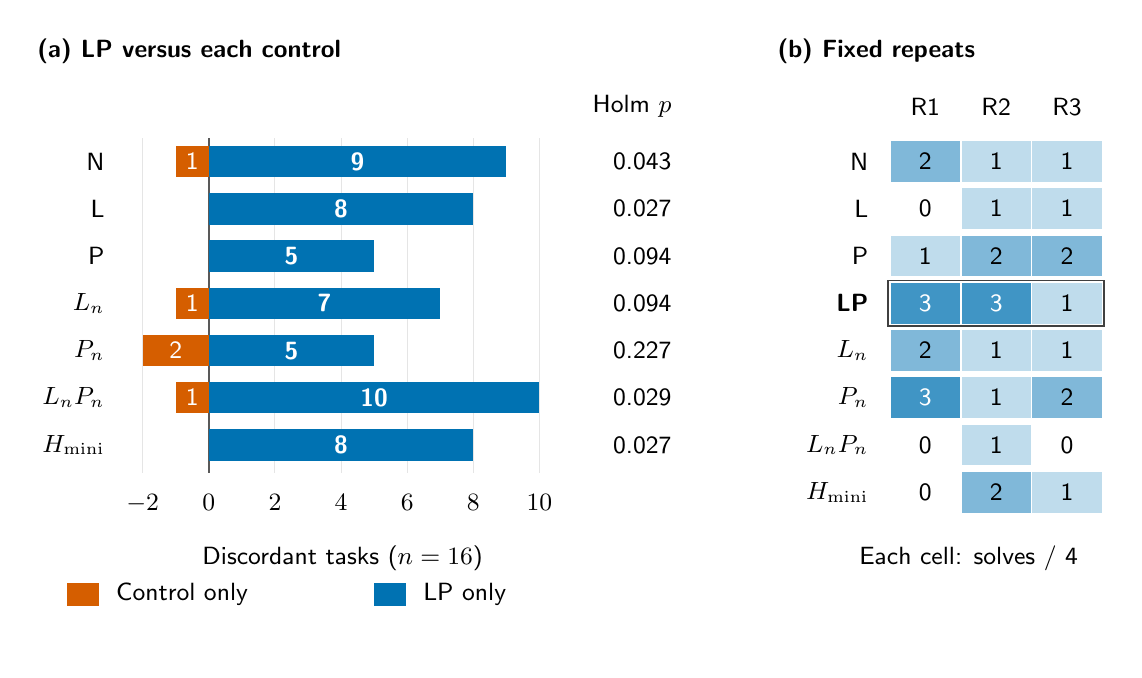
\begin{tikzpicture}[x=1mm,y=1mm,font=\sffamily\fontsize{9}{10.5}\selectfont]
\path[use as bounding box] (0,0) rectangle (138,79);
\node[anchor=west,font=\sffamily\bfseries\fontsize{9.5}{11}\selectfont] at (0,76) {(a) LP versus each control};
\node[anchor=west,font=\sffamily\bfseries\fontsize{9.5}{11}\selectfont] at (94,76) {(b) Fixed repeats};
\node[anchor=east] at (83,69) {Holm $p$};
\foreach \value in {-2,0,2,4,6,8,10}{
  \draw[black!10,line width=.4pt] ({23+4.2*\value},22.5)--({23+4.2*\value},65);
  \node[anchor=north] at ({23+4.2*\value},21) {$\value$};
}
\draw[black!65,line width=.55pt] (23,22.5)--(23,65);
\pairrow{62}{N}{9}{1}{0.043}
\pairrow{56}{L}{8}{0}{0.027}
\pairrow{50}{P}{5}{0}{0.094}
\pairrow{44}{$L_n$}{7}{1}{0.094}
\pairrow{38}{$P_n$}{5}{2}{0.227}
\pairrow{32}{$L_nP_n$}{10}{1}{0.029}
\pairrow{26}{$H_{\mathrm{mini}}$}{8}{0}{0.027}

\node at (114,69) {R1};
\node at (123,69) {R2};
\node at (132,69) {R3};
\repeatrow{62}{N}{2}{1}{1}
\repeatrow{56}{L}{0}{1}{1}
\repeatrow{50}{P}{1}{2}{2}
\repeatrow{44}{\textbf{LP}}{3}{3}{1}
\repeatrow{38}{$L_n$}{2}{1}{1}
\repeatrow{32}{$P_n$}{3}{1}{2}
\repeatrow{26}{$L_nP_n$}{0}{1}{0}
\repeatrow{20}{$H_{\mathrm{mini}}$}{0}{2}{1}

\draw[black!75,line width=.65pt] (109.3,41.1) rectangle (136.7,46.9);
\node[anchor=north] at (40,14.5) {Discordant tasks ($n=16$)};
\fill[Loss] (5,5.5) rectangle (9,8.5);
\node[anchor=west] at (10,7) {Control only};
\fill[Benefit] (44,5.5) rectangle (48,8.5);
\node[anchor=west] at (49,7) {LP only};
\node[anchor=north,align=center] at (119.5,14.5) {Each cell: solves / 4};
\end{tikzpicture}
\end{document}
